\chapter{Background}\label{ch:background}
% Outline for the section:
% - Network Side Channels
% 	- Overview
% 	- Target application: Video Streaming
% 	- CNN classifier (BB)

% - Defenses
% 	- Path splitting approaches
% 	- Adversarial ML approaches
% 	- Shaping based approaches
% 		- Static shaping
% 		- Dynamic shaping

% - Differential Privacy Overview

% - QUIC Overview (I am not convinced yet this is necessary.)

% - Threat Model
% Background intro. Explaining what you've included in this section. 
% TODO: update if you add more to background

We begin this chapter by discussing the problem of network side-channel attacks in \Cref{sec:ns-attacks}, in the context of two distinct applications: video streaming and web services.
In \Cref{sec:dp-background}, we present a comprehensive definition of differential privacy (DP), outline its key properties, and highlight its primary applications, thereby setting the foundation for our differentially private traffic shaping mechanism.
In \Cref{sec:background-quic} we provide a brief overview of the QUIC protocol, which plays a pivotal role in the design of {\sys}.
Finally, in \Cref{sec:threat-model}, we conclude this chapter by explaining our threat model. 

\section{Network Side-Channel Attacks}\label{sec:ns-attacks}
% What is a side channel?
In this section, we provide an overview of network side-channel attacks. 
We, further, discuss video streaming as one specific target application of side-channel attacks, and explain the state-of-the-art traffic analysis attack proposed for this application and elaborate on its strengths and weaknesses. 

A side channel is a method of extracting information from a program by observing its functionality and environment, rather than through its intended input or output. 
Extracting information from side channels becomes particularly viable when a program has shared resources with other untrusted entities. 
When an adversary shares resources with the victim's program, it can observe victim's resource usage pattern.
The adversary then can leverage the correlation between resource usage pattern (side channels) and victims' secrets to breach their privacy.

% Essential Steps in side channel attacks
A side-channel attack comprises two essential steps: Profiling and Inference.
During profiling, the adversary extracts the correlation between the victim's secrets and their resource usage patterns.
This involves monitoring various resource usage patterns that emerge during the program's execution.
In the inference step, the adversary utilizes the prior knowledge acquired in the first step to infer the victim's secrets based on the observations of resource usage patterns.
One trivial solution to address side-channel attack is to isolate the program and all its dedicated resources such as CPUs, memory, storage, and network resources at all possible level down to hardware. 
However, this approach often results in inefficient resource utilization, as the resources that the program does not currently use remain idle. 
Moreover, many programs rely on inherently shared resources, such as a common network infrastructure.
Therefore, mitigating side-channels attacks is intrinsically challenging. 

% What are network side channels 
Network applications, such as web browsers, email clients, video conferencing software, file-sharing services, and online gaming platforms, are exceedingly popular these days.
These applications consist of a service that communicates with clients over an encrypted communication on the network.
However, the encryption does not conceal packet sizes and timing transmitted by an application, which is correlated with users' sensitive information in many applications.
In a network side-channel attack, by utilizing this correlation, an adversary with control over the underlying network links (e.g., Internet Service Providers) can monitor the traffic pattern and potentially reveal the content of the communication.
Recent advancements in machine learning have significantly empowered the inference step of network side-channel attacks, providing adversaries with enhanced capabilities to effectively map observations to the victim's sensitive information~\cite{schuster2017beautyburst, bhat2019varcnn, hayes2016kfp, sirinam2018df}.


% \subsection{Website Fingerprinting}\label{subsec:web-fingerprinting}

\subsection{Video identification}\label{subsec:video-classification}
Recently, video services have gained immense popularity, becoming an integral part of people's daily Internet activities.
Video-sharing platforms, such as YouTube, and commercial online streaming platforms, such as Netflix, constitute a significant portion of the world's total network traffic.
In 2023, video services account for 82.5\% of all web traffic, making them by far the most popular type of content over the internet~\cite{webstat}.
The popularity of these services makes them a natural target for traffic analysis attacks.
Video streams are characterized by bursty traffic patterns, which often involves short-lived periods of high rate data transmission interspersed with relatively longer periods of low or moderate rate network activity.
When these patterns are correlated with specific content, an adversary capable of measuring them may have the ability to identify the exact video being streamed.
In this section, we first provide an overview of the widely used video streaming protocol, Dynamic Adaptive Streaming over HTTP (MPEG-DASH), and examine how it can potentially result in information leakage. 
Next, we elaborate on the state-of-the-art network side-channel attack, known as Beauty and the Burst~\cite{schuster2017beautyburst}, which leverages bursty pattern of MPEG-DASH protocol to reveal users' information. 

In MPEG-DASH protocol, the video server encodes the video content and divide it into short segments, ranging from few seconds to few tens of seconds.
Then, it creates a Manifest file to store information about available data segments, their quality, and a URL to access them.
Upon receiving a request for a video from a client, the video server sends the Manifest file to the client. 
Following this, the client sends requests based on the URLs provided in the Manifest file to download segments corresponding to the desired quality.
The segment sizes and the timing of each segment can collectively create a unique pattern for a video.
An adversary with control over network link can measure segment sizes and their temporal pattern to identify the streaming video.
In Beauty and the Burst paper~\cite{schuster2017beautyburst}, the authors show that even a malicious extension in a browser, can extract segment sizes and timing of a video that the user is watching.
Based on the MPEG-DASH standard, Beauty and Burst attack model traffic traces as time-series.
Specifically, each traffic segment can be represented as a tuple $(t_i, b_i)$, where $t_i$ denotes the segment's transmission time and $b_i$ represents its size. 
A traffic analysis attack involves the attempt to infer the content of traffic from its observed pattern, which is essentially a sequence modeling task.
At the inference stage, Beauty and the burst~\cite{schuster2017beautyburst} utilizes a convolutional neural network (CNN) architecture to classify videos based on the time-series representation of observed traffic.
The architecture of Burst and Beauty model is represented in \Cref{fig:bandb-arch}. 
We evaluate this architecture with our dataset in section {\addref}.
\begin{figure}[t]
  \centering
  %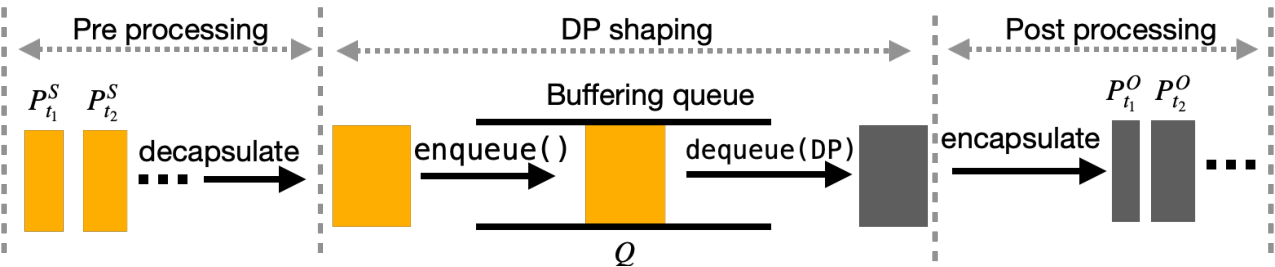
\includegraphics[width=\columnwidth]{figures/DPshaping_concept_vertical.pdf}
  %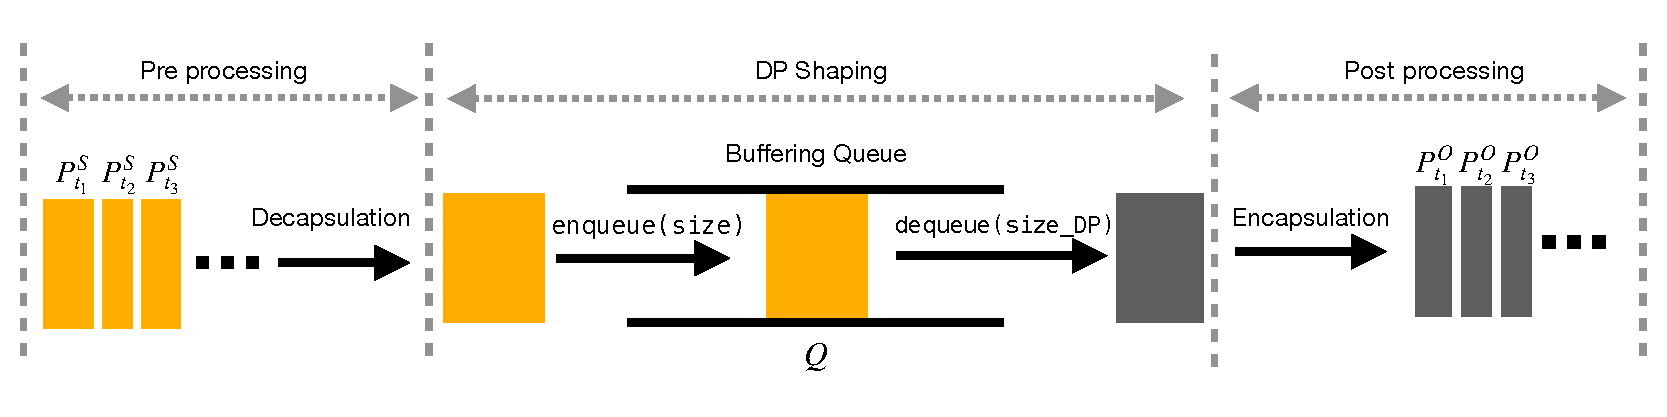
\includegraphics[width=\columnwidth]{figures/DPshaping_concept_horizontal.pdf}
  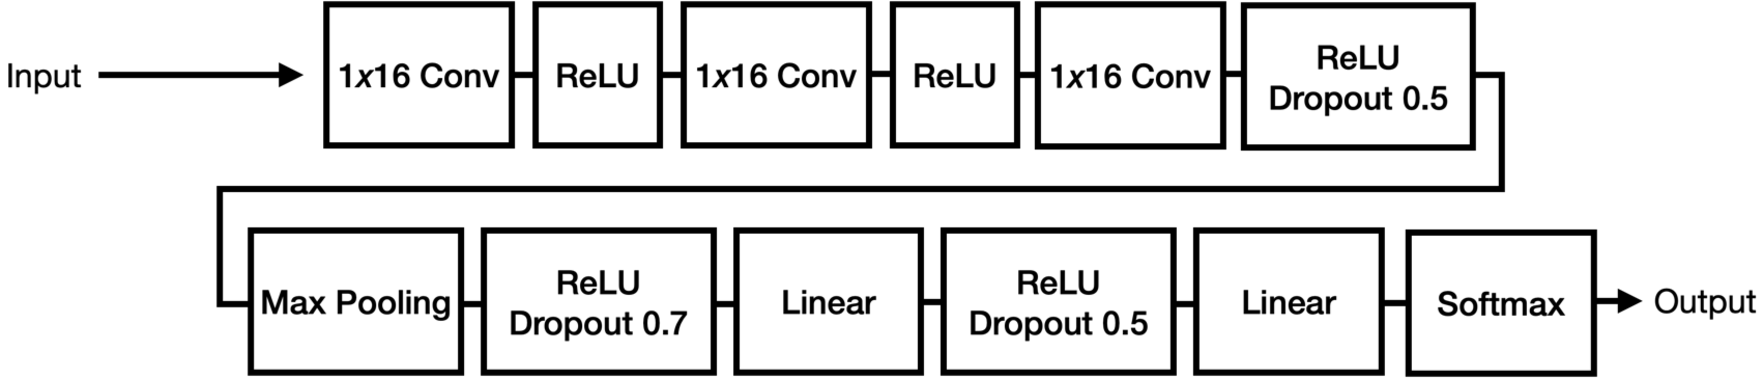
\includegraphics[width=\columnwidth]{figures/BandB_arch.pdf}
  \caption{Beauty and The Burst CNN model architecture.}
  \label{fig:bandb-arch}
\end{figure}


\subsection{TCN-based Video identification}
\todo{Move it to somewhere else to highlight that it is your contribution}
Beauty and the Burst~\cite{schuster2017beautyburst} uses a CNN-based architecture to for video identification. 
Convolutional neural networks have been shown to be effective in sequence modeling for decades~\cite{hinton1990connectionist}.
However, there are two problems with using a convolutional neural network as a sequence modeler.
First, convolutional layers applied to a sequence are not inherently causal, meaning that they look into future samples of a sequence to decide the output for the current sample.
Secondly, in contrast to recurrent neural networks(RNNs)~\cite{elman1990finding}, convolutional neural networks lack a deep effective history size of past samples in the sequence (i.e. their effective history is bounded to the number of samples that kernel can cover from the past).
To address these problems, Bai\etalc{bai2018empirical} proposed a new architecture called Temporal Convolutional Network (TCN).
The TCN utilizes a one-dimensional fully-convolutional network~\cite{long2015fully} equipped with causal dilated convolutions~\cite{oord2016wavenet}, allowing it to examine deep into the past to produce an output for the sequence at any given moment.
They added a generic residual block from input to output.
The architecture is shown in the \Cref{fig:tcn-arch}.
We evaluate the effectiveness of TCN model for network side-channel attacks in {\addref}




\begin{figure}[t]
  \centering
  %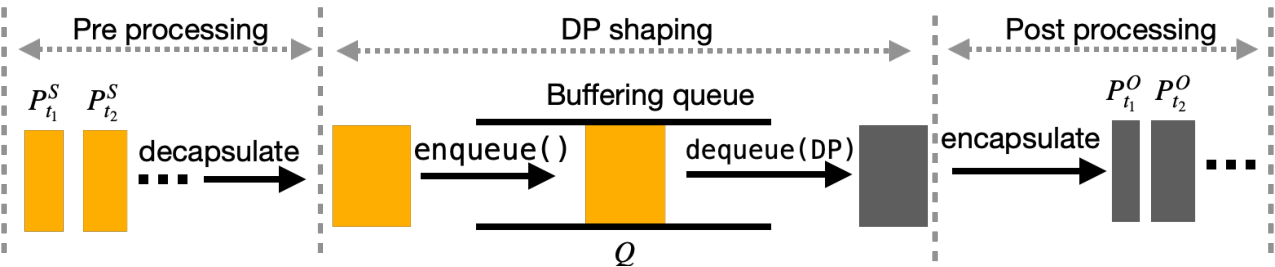
\includegraphics[width=\columnwidth]{figures/DPshaping_concept_vertical.pdf}
  %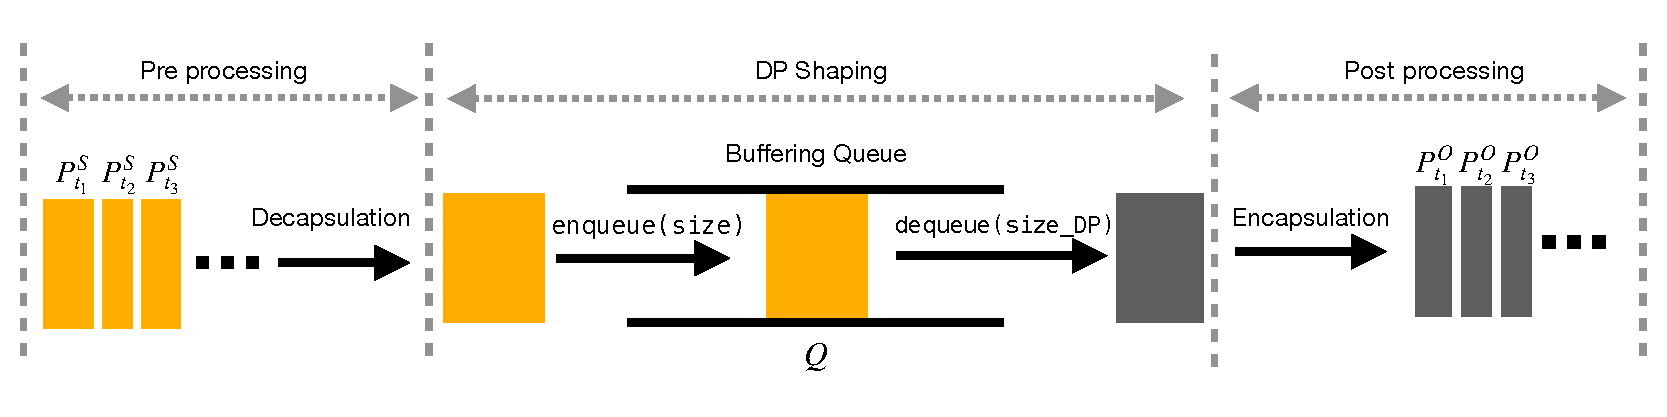
\includegraphics[width=\columnwidth]{figures/DPshaping_concept_horizontal.pdf}
  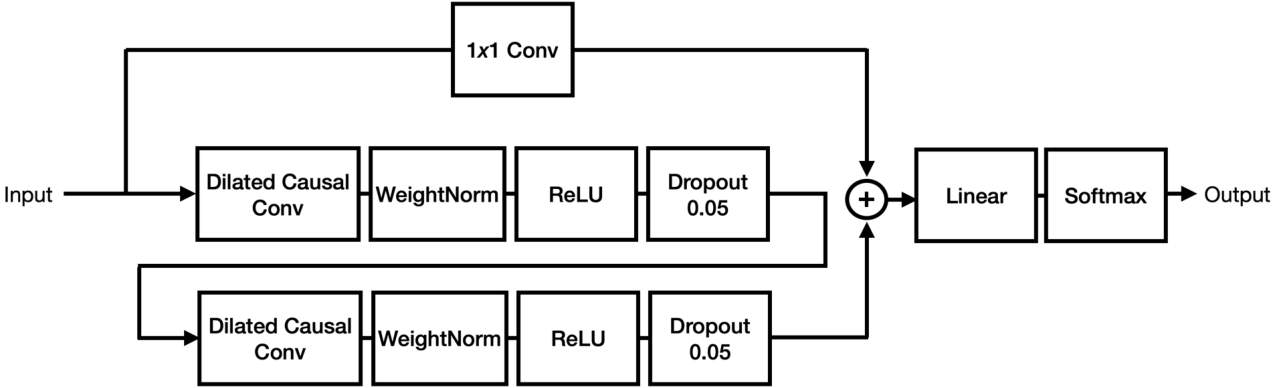
\includegraphics[width=\columnwidth]{figures/TCN_arch.pdf}
  \caption{TCN model architecture.}
  \label{fig:tcn-arch}
\end{figure}


\section{Differential Privacy}\label{sec:dp-background}
% Subsection intro. Elaborate on origins of DP. Why it is useful.
Data scientists always strive to understand the general properties of a population. 
To answer questions concerning the etiology of a disease, factors contributing to a societal phenomenon, or the consequences of an economic policy, researchers collect data from individual people. They then process this data to calculate population-level statistics and propose solutions based on these aggregated statistics.
Ensuring the privacy of individuals who have contributed to these studies is of utmost importance from both ethical and legal perspectives.
In fact, the intended goal of all scientific studies is to collect valuable information about the targeted population not individual people within the population. 
However, it is impossible to learn useful information about a population while learning \textit{nothing} about individuals, leading to a paradox between usefulness of a dataset (\ie utility) and its privacy. 
Differential Privacy (DP) addresses this paradox by quantifying the extent of privacy leakage for individuals in a dataset when publishing its statistics.
Within the framework of Differential Privacy (DP), the aforementioned paradox transforms into an adjustable trade-off between the utility of data and the preservation of privacy. 

In the rest of this section, we provide the formal definition of differential privacy, highlight its main properties, and explore its potential application in the domain of traffic shaping.


%
%% 
%% Definition
%%
%


\subsection{Definitions}\label{subsec:background-dp-definitions}
A database $D$ has a fixed number of entries, where each individual data point is stored in one entry.
Following the notation proposed by Dwork \etal \cite{dwork2014algorithmic}, we represent databases by their histograms: $D \in \dbSpace$. 
In this representation, every entry $D_i$ of the database $D$ represents the number elements of type $i \in \mathcal{X}$.
\\  
Within the DP context, we define a \textit{query} as a function that operates on a database. 
Any computation performed on a database, regardless of its codomain, can be regarded as a query executed on that database.
The primary objective of differential privacy is to offer meaningful population-level information for queries executed on a database, all while protecting the privacy of individual data points within the database.
Intuitively, small changes in a database should not significantly impact the outcome of a query.
To further clarify the terms "small changes" and "significant impact", we provide definitions for neighboring databases and query function sensitivity, respectively.
\\
We measure the difference between two databases with a distance metric $\rho(D, D')$.
\begin{definition}[Neighboring databases]
  Given a distance metric $\rho$, we refer to two databases $D, D' \in \dbSpace$ as neighboring databases, if and only if $\rho(D, D') \leq 1$.             
\end{definition}
\noindent In the standard DP definition, the distance metric is simply the number of different data entries in two databases (\ie Hamming distance).
However, Chatzikokolakis \etal \cite{chatzikokolakis2013broadening} show that DP applies to a general definition of distance metrics.
\\
To quantify the extent to which a single data point can influence the outcome of a query in worst-case, we introduce the concept of sensitivity. 
\begin{definition}[$l_p$-Sensitivity]
  \label{def:norm-sensitivity}
  The $l_p$-sensitivity of a query function $f$ is:
  \begin{equation*}
    \Delta_p f = \max_{D, D'} \|f(D) - f(D')\|_p 
  \end{equation*}
where $\rho(D, D') \leq 1$ (\ie $D$ and $D'$ are neighboring databases).
\end{definition}
\noindent
Differential Privacy involves randomization of query outputs. We define a randomized algorithm as follows.
\begin{definition}[Randomized algorithm]
  \label{def:randomized-algorithm}
  A randomized algorithm $M$ with the domain $A$ and discrete range $B$, for any given $a \in A$ and $b \in B$ outputs $M(a)= b$ with probability of $(M(a))_b$.
\end{definition}

With all the necessary components in place, we are now prepared to present the formal definition of differential privacy.
\begin{definition}[Differential privacy]
  \label{def:dp}
  A randomized algorithm $M: \dbSpace \rightarrow \mathbb{R}$ is $(\varepsilon, \delta)$-differentially private if for all ${S} \subseteq Range(M)$ and for  all $D, D' \in \dbSpace$ such that $\rho(D, D') \leq 1$, we have:
  \begin{equation*}
    \Pr[M(D) \in S] \leq \exp(\varepsilon)\Pr[M(D') \in S] + \delta
  \end{equation*}
\end{definition}
\noindent
Indeed, Differential Privacy (DP) is a definition rather than a specific algorithm.
It provides a framework for ensuring privacy guarantees in various randomized algorithms. Multiple randomized algorithms can achieve $(\varepsilon, \delta)$-privacy for a given set of databases, each with different characteristics. 
Intuitively, given an output, with probability $1-\delta$ the log likelihood ratio of running the algorithm $M$ on databases $D$ and $D'$ is bounded by $\varepsilon$.
This bound ensures that the presence or absence of any individual's data in the database has a limited impact on the likelihood of obtaining a particular output.
The smaller $\varepsilon$ implies that both neighboring databases are equally likely to generate the output, resulting in more privacy.
The parameter $\varepsilon$ is commonly referred to as \textit{privacy loss} within the context of DP.
The parameter $\delta$ determines the failure probability of a differential private mechanism and is typically expected to have a small value (\ie smaller than $10^{-5}$).


%
%% 
%% Properties
%%
%

\subsection{Properties}\label{subsec:background-dp-properties}
In this section, we explore the key properties of Differential Privacy as a privacy framework.


% ROBUSTNESS TO AUXILIARY INFORMATION.
\subsubsection{Robustness to auxiliary information}
\label{subsubsec:dp-auxiliary}
The definition of Differential Privacy does not make any assumptions regarding the prior knowledge of the adversary. 
In other words, regardless of the adversary's prior knowledge, the information gained by the adversary after observing the output of a differentially private algorithm $M$ remains within the bounds specified by Differential Privacy. 
\begin{proposition}
  \label{prop:auxiliary}
  Assume that the adversary has a prior $\Pr(D)$ over the set of all possible databases $D, D' \in \dbSpace$, given the output $S$ of a $(\varepsilon, \delta)$-DP algorithm $M: \dbSpace \rightarrow \mathbb{R}$, for all $D, D' \in \dbSpace$ such that $\rho(D, D') \leq 1$, we have: 
  \begin{equation*}
    \frac{\Pr(D|S)}{\Pr(D'|S)} \leq \exp(\varepsilon) \frac{\Pr(D)}{\Pr(D')}
  \end{equation*}
\end{proposition}
In broad terms, robustness to auxiliary information in the context of Differential Privacy is similar to the security semantics of cryptographic algorithms. 
For instance, consider a scenario where an adversary possesses the knowledge that the content of an encrypted message is either a picture of a car or a picture of a tree.
In this case, observing the encrypted message does not provide any additional evidence to indicate which of the two possibilities is more likely to be the true message.
In DP, nevertheless, observing the results of private queries does change the prior knowledge of the adversary.
However, this change remains within the boundaries defined by DP and does not exceed them.

% POST-PROCESSING
\subsubsection{Post-processing}
\label{subsubsec:background-dp-postprocessing}
Differential Privacy guarantees are resilient to post-processing of the output from a DP algorithm.
In fact, in the absence of any additional knowledge, the adversary is unable to undermine the guarantees of Differential Privacy simply by processing the output of the algorithm.
\begin{proposition}
  \label{prop:post-processing}
  Consider $M: \dbSpace \rightarrow R$ as a $(\varepsilon, \delta)$-differentially private algorithm, and let $g: \mathbb{R} \rightarrow \mathbb{R}$ be an arbitrary randomized mapping, then $g(M(.)): \dbSpace \rightarrow \mathbb{R}$ is $(\varepsilon, \delta)$-differentially private. 
\end{proposition}
\noindent
This implies that regardless of the complexity of a procedure, as long as the inputs are differentially private, the output is guaranteed to maintain the same level privacy.
The post-processing property of Differential Privacy can be especially advantageous when dealing with systems that have information bottlenecks, such as situations where results from multiple calculations are aggregated at a single stage.
In such systems, by applying a differentially private algorithm to the information bottleneck, the guarantee of Differential Privacy extends to the output of the entire system. 
We specifically utilize post-processing property of Differential Privacy in the design of both the {\sys} shaping mechanism and the {\sys} middlebox. 

% PRESERVATION UNDER ADAPTIVE SEQUENTIAL COMPOSITION.
\subsubsection{Self-Composition}\label{subsubsec:background-dp-composition}
The simultaneous release of results from multiple differentially private algorithms maintains the differential privacy guarantee.
This property facilitates the modular construction of differentially private algorithms, allowing multiple DP algorithms to be combined to create more sophisticated and advanced algorithms.
Furthermore, the composition theorem enables us to compute the privacy parameters associated with the sequential release of a differentially private algorithm output, thereby facilitating multiple releases of the same DP output.
There are multiple variants of composition theorem, and we with the simplest form of composition.
\begin{proposition}[Basic composition theorem]
\label{prop:basic-composition}
  Let $M_i: \dbSpace \rightarrow \mathbb{R}$ be an $(\varepsilon_i, \delta)$-differentially private algorithm for $i \in [k]$. Then, the combination of these $k$ algorithms, $M_{[k]}: \dbSpace \rightarrow \Pi_{i=1}^{k}\mathbb{R}$ is $(\sum_{i=1}^{k}\varepsilon_i, \sum_{i=1}^{k}\delta_i)$-differentially private.  
\end{proposition}
Basic composition theorem states that the privacy loss resulting from the combination of multiple differentially private algorithms is equal to the aggregate of their individual privacy losses.
While functional, the basic composition theorem tends to overestimate the privacy loss of combined DP algorithms.
The advanced composition theorem offers a more precise and rigorous bound for the aggregated privacy loss incurred by multiple differentially private algorithms. 
\begin{proposition}[Advanced composition theorem]
\label{prop:advanced-composition}
  Let $M_i: \dbSpace \rightarrow \mathbb{R}$ be an $(\varepsilon, \delta)$-differentially private algorithm for $i \in [k]$. Then, the combination of these $k$ algorithms, $M_{[k]}: \dbSpace \rightarrow \Pi_{i=1}^{k}\mathbb{R}$ is $(\varepsilon', k\delta+\delta')$-differentially such that:
  \begin{equation*}
    \forall \delta' \geq 0: \varepsilon' = \sqrt{2k\ln(1/\delta')}\varepsilon + k\varepsilon(e^{\varepsilon} - 1)
  \end{equation*}
\end{proposition}
It is important to note that this form of composition theorem is only applicable to differentially private algorithms that share the same privacy parameters.
More sophisticated versions of the composition theorem exist, offering tighter privacy bounds~\cite{kairouz2015composition, mironov2017renyi}.
We particularly use R{\'e}nyi Differential privacy to calculate the privacy loss of our differentially private shaping mechanism.

\subsection{Mechanisms}\label{subsec:background-dp-mechanism}
\Cref{def:randomized-algorithm} provides a general definition of a randomized algorithm, while \Cref{def:dp} outlines the specific criteria that a randomized algorithm must satisfy to be considered differentially private (\ie DP mechanism).
In this section, we will explore the two most commonly used differentially private mechanisms: the Laplace mechanism and the Gaussian mechanism\cite{dwork2014algorithmic}.
\begin{definition}[Laplace Mechanism]\label{def:laplace-mechanism}
  Given any function $f: \dbSpace \rightarrow \mathbb{R}^k$ the Laplace mechanism is defined as:
  \begin{equation*}
    \mathcal{M}(x, f, \varepsilon) = f(x) + (Y_1, Y_2, \dots, Y_k)
  \end{equation*}
  where $Y_i$ are i.i.d random variables from Laplace distribution with probability density function of $Lap(\Delta_1 f/\varepsilon)$, and $\Delta_1 f$ is $l_1$-sensitivity of function $f$ (see \Cref{def:norm-sensitivity}).
\end{definition}
The Laplace mechanism is relatively easy and straightforward. 
Intuitively, it just adds a random variable driven from a Laplace distribution to the result of the query.
The variance of this random variable quantifies the privacy of query results, as a higher variance makes it more challenging for adversaries to infer the true result of the query.
\begin{proposition}
  The Laplace mechanism of \Cref{def:laplace-mechanism} is $(\varepsilon, 0)$-differentially private. 
\end{proposition}
\noindent
We omit the proof here; you can refer to the work of Dwork\etalc{dwork2014algorithmic} for a detailed proof. 
As we can see in \Cref{def:laplace-mechanism}, the failure probability of Laplace mechanism, $\delta$, is 0.
In broad terms, a mechanism can compromise failure rate $\delta$ to add less noise to query results while achieving same values for privacy loss $\varepsilon$.
\begin{definition}[Gaussian Mechanism]\label{def:gaussian-mechanism}
  Given any function $f: \dbSpace \rightarrow \mathbb{R}^k$ the Gaussian mechanism is defined as:
  \begin{equation*}
    \mathcal{M}(x, f, \varepsilon, \delta) = f(x) + (Y_1, Y_2, \dots, Y_k)
  \end{equation*}
  where $Y_i$ are i.i.d random variables from Gaussian distribution $\mathcal{N}(0, \frac{2\Delta_2 f^2}{\varepsilon^2})\ln(\frac{1.25}{\delta})$, and $\Delta_2 f$ is $l_2$-sensitivity of function $f$ (see \Cref{def:norm-sensitivity}).
\end{definition}
We particularly design our differentially private traffic shaping mechanism using Gaussian mechanism at its core. 
We elaborate on this in \Cref{subsec:dp-shaping-mechanism}.

\subsection{R\'enyi Differential Privacy}
Despite widespread usage, straightforward interpretability,, and numerous applications of standard definition of $(\varepsilon, \delta)$-differential privacy, this concept does exhibit two primary limitations. 
First, the presence of the failure probability $\delta$ in this definition contradicts the guarantee of  plausible deniability associated with differential privacy since with probability $\delta$ the secret can be completely exposed.    
Secondly, as we mentioned in \Cref{subsec:background-dp-properties}, the desirable results of strong composition theorem only holds for homogeneous DP mechanisms.
In fact, Vadhan~\etalc{murtagh2015complexity} demonstrate that the generalization of advanced composition theorem to heterogeneous DP mechanisms (\ie $(\varepsilon_i, \delta_i)$-DP for different values of $\varepsilon_i$ and $\delta_i$) is P-hard.
To address these limitations, Mironov~\etalc{mironov2017renyi} propose a new definition of differential privacy based on the R\'enyi divergence~\cite{renyi1961measures}.
R\'enyi differential privacy (RDP) is strictly stronger than $\varepsilon, \delta$-DP, meaning that any $\varepsilon, \delta$-DP mechanism is RDP though the reverse does not hold true.
In this section, we explain the core concepts of R\'enyi differential privacy (RDP), elaborate on its properties, and highlight its connection to standard definition of DP.

\begin{definition}[R\'enyi divergence]
  for two probability distributions $P$ and $Q$, the R\'enyi divergence of order $\alpha > 1$ is defined as:
  \begin{equation*}
    D_{\alpha}(P||Q) \triangleq \frac{1}{\alpha-1} \log E_{x \sim Q}\left ( \frac{P(x)}{Q(x)} \right )
  \end{equation*}
\end{definition}
R\'enyi divergence simply measure the difference between two distributions $P$ and $Q$.
For $\alpha = \infty$, the R\'enyi divergence specifically defined as:
\begin{equation*}
  D_{\infty}(P||Q) \triangleq  \sup_{x \sim Q} \; \log \left ( \frac{P(x)}{Q(x)} \right ) 
\end{equation*}
We can see that the R\'enyi divergence with $\alpha=\infty$ is closely connected to $(\varepsilon, 0)$-DP definition.
\begin{proposition}
  A randomized algorithm $M: \dbSpace \rightarrow \mathbb{R}$ is $(\varepsilon, 0)$-differentially private iff for all $D, D' \in \dbSpace$ such that $\rho(D, D') \leq 1$, we have:
  \begin{equation*}
    D_{\infty}(P||Q) \leq \varepsilon
  \end{equation*} 
\end{proposition}
\noindent Next, we provide the formal definition of R\'enyi DP.
\begin{definition}[$(\alpha, \varepsilon)$-RDP]
  A randomized algorithm $M: \dbSpace \rightarrow \mathbb{R}$ is $(\alpha, \varepsilon)$-RDP if for all $D, D' \in \dbSpace$ such that $\rho(D, D') \leq 1$, we have:
  \begin{equation*}
    D_{\alpha}(\mathcal{M}(D)||\mathcal{M}(D')) \leq \varepsilon
  \end{equation*}
\end{definition}
\noindent Indeed, all the favorable attributes of the standard definition of differential privacy, including post-processing, self-composition, and robustness to auxiliary information, remain applicable to R\'enyi differential  privacy.
Particularly, the composition theorem has a simple representation in RDP.
\begin{proposition}[R\'enyi Composition]\label{prop:rdp-composition}
  Let $M_i: \dbSpace \rightarrow \mathbb{R}$ be an $(\alpha, \varepsilon_i)$-RDP algorithm for $i \in [k]$. Then, the combination of these $k$ algorithms, $M_{[k]}: \dbSpace \rightarrow \Pi_{i=1}^{k}\mathbb{R}$ is $(\alpha, \sum_{i=1}^{k}\varepsilon_i)$-RDP.   
\end{proposition}
\noindent For an in-depth proof, we direct readers to the R\'enyi differential privacy paper~\cite{mironov2017renyi}.
So far, we explained three methods to calculate the aggregated privacy loss of multiple releases of differentially-private mechanism.
These methods are basic composition theorem, advanced combination theorem, and R\'enyi composition theorem.
The goal of these methods is to provide a tight, accurate bound on aggregated privacy loss without overestimation. 
In simpler terms, a composition theorem is superior to another, if it can provably show that the aggregated privacy loss of a differentially-private mechanism, after multiple release of results, is smaller than the aggregated privacy loss indicated by the other mechanism.
A natural question is: \textit{What is the difference between all these mechanisms?}
To answer these questions, we calculate the privacy loss reported by these mechanisms for different number of queries (\ie varying number of differentially-private releases of results).
We fix epsilon and delta per query $0.2$ and $0.0001$ respectively, and report the final privacy loss for a given number of queries.
\begin{figure}[t]
  \centering
  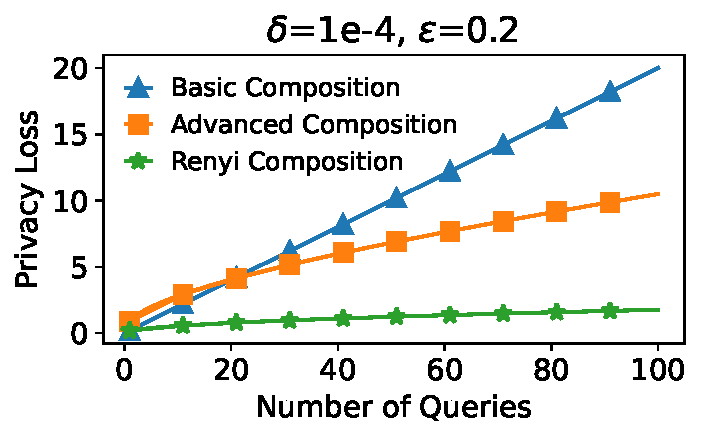
\includegraphics[width=\columnwidth]{plots/composition_comparison.pdf}
  \caption{Aggregated privacy loss of multiple queries reported by different composition methods}
  \label{fig:composition-comparison}
\end{figure}

\Cref{fig:composition-comparison} compares different methods for composing privacy loss of DP mechanisms.
We can see the effectiveness of R\'enyi methods as compared to others across all values for number of queries.
Advanced composition theorem also outperforms basic composition theorem for larger number of queries. 


As we mentioned earlier, $(\alpha, \varepsilon)$-RDP is strictly stronger than $\varepsilon, \delta$-DP. 
Next proposition shows how RDP implies standard DP.
\begin{proposition}\label{prop:rdp-better-than-dp}
  If $M: \dbSpace \rightarrow \mathbb{R}$ is an $(\alpha, \varepsilon)$-RDP mechanism, it is also $(\varepsilon + \frac{\log 1/\delta}{\alpha-1}, \delta)$-DP for any $0 < \delta < 1$. 
\end{proposition}
\noindent \Cref{prop:rdp-better-than-dp} enables us to interpret guarantees of R\'enyi differential privacy with semantics of standard differential privacy. 
Besides that, \Cref{prop:rdp-composition} provides us with the means to compose heterogeneous differentially private algorithms, while and at the end, with \Cref{prop:rdp-better-than-dp} we can still represent the final result using semantics of standard DP. 
In order to compute the privacy loss (\ie $\varepsilon$) of our differentially private shaping mechanism in \Cref{sec:dp-privacy-guarantees}, we use \Cref{prop:rdp-composition} referred to as $\textrm{DP\_compose}()$.

\section{QUIC Transport Protocol}\label{sec:background-quic}

QUIC is a modern transport layer protocol specifically developed to enhance the performance of HTTPS traffic~\cite{langley2017quic}.
In the traditional IP stack model, QUIC encompasses both the Transport layer and the Application layer.
In other words, QUIC is a user-space transport layer protocol built on top of UDP. 
Using UDP packets as the transport layer carrier allows QUIC packets to traverse current network infrastructure developed for TCP/UDP protocols such as middleboxes.
On the top of UDP, QUIC provides transport functionalities of flow control, loss recovery, encryption, and congestion control.
Unlike TCP, QUIC mitigates head-of-the-line blocking delays by introducing a novel data structuring abstraction known as streams. 
QUIC is now standardized under RFC 9000~\cite{rfc9000}, and the details of design and implementation of the protocol is well beyond the scope of this thesis.
We, however, provide a brief overview of QUIC features and functionalities that are relevant to the design of {\sys}.




\subsection{QUIC Connections}
A QUIC connection is a shared state between a client and a server.
At the initiation of each connection, a handshake phase takes place where the two endpoints engage in a cryptographic handshake protocol~\cite{rfc9001} to establish a shared secret and negotiate the application protocol.
This handshake process ensures mutual consent for communication and establishes connection parameters.

Each connection has two unique IDs, source connection ID, and destination connection ID.
By assigning each connection unique identifiers (ID), the potential changes in addressing layers at lower network levels, such as UDP and IP, do not result in incorrect packet delivery at the receiving endpoint.
Furthermore, routers can leverage existence of destination connection ID to route QUIC packets in the network to the correct endpoint.
During the handshake, one endpoint establishes the Source Connection ID by setting it in the packet header.
Similarly, the other endpoint determines the Destination Connection ID.

QUIC provides three ways to terminate a connection: idle timeout, immediate close, and stateless reset.
Each endpoint can specify an idle timeout in its transport parameters.
If the idle timeout duration elapses without any data exchange between the endpoints, the endpoint will silently close the connection (\ie without explicitly notifying the other endpoint). 
The other connection termination method is the immediate close. 
To promptly terminate the connection, an endpoint transmits \texttt{CONNECTION\_CLOSE} frame. 
This frame triggers the immediate termination of all streams within the connection.
Upon sending a \texttt{CONNECTION\_CLOSE} frame, the sender promptly terminates the connection without waiting for acknowledgment from the receiver.
A stateless reset is available as a fallback choice for an endpoint that lacks access to the connection state.
In cases of a crash or outage, it is possible for endpoints to continue sending data to an endpoint that cannot properly maintain the connection.
In such cases, the endpoint without the connection state issues the stateless reset, terminating the connection and its state machine locally.




\subsection{QUIC Streams}
QUIC's streams offer a lightweight and ordered way for applications to send byte-streams.
These streams can be either unidirectional or bidirectional, depending on the specific needs of the application.
Within a connection, each stream is identified with a new ID.
A stream ID is 62 bit integer.
Either of endpoints can create a stream just by sending data with a new stream ID. 
There are no restrictions on the number of simultaneous streams (other than, of course, the maximum number of unique IDs) or the length of each individual stream.
QUIC assigns different priorities to different streams based on the applications' requirement.
The prioritization of streams within a connection can have a substantial impact on the performance of applications.
Each stream has a dedicated header with 5 major fields: Type, Stream ID, Offset, and Data Length.
The stream header within a packet is encrypted, ensuring that adversaries are unable to discover the active streams in a connection.
Either of endpoints can terminate streams by sending a \texttt{STREAM\_RESET} frame to the other one.
In a bidirectional stream, both endpoints should send \texttt{STREAM\_RESET} message to completely terminate a stream.

% \subsection{QUIC Congestion and Flow Control}
% \subsubsection{Flow Control}
% To prevent a fast or malicious sender from overwhelming receivers' buffer, receivers must proactively limit the amount of data a sender can send.
% QUIC can perform flow control at two levels: The receiver controls the maximum amount of data the sender can send on a per-stream basis, as well as across all streams within a connection. 
% The receiver sets the initial limits for stream and connection flow controls during the handshake. 
% During the handshake, the receiver establishes the initial limits for both stream and connection flow controls. Throughout the connection, if the receiver needs to adjust the limits for a specific stream, it sends \texttt{MAX\_STREAM\_DATA} frames to the sender.
% Similarly, to change the limit for overall connection, the receiver sends \texttt{MAX\_DATA} frames to the sender.

% \subsubsection{Congestion Control}
% QUIC does not standardize any specific method of congestion control.
% Instead, it provides the necessary feedback mechanism to implement congestion control.
% The modular design of congestion control makes QUIC more flexible, allowing applications to implement a congestion mechanism that aligns with their specific requirements.
% As the default congestion control mechanism, however, QUIC uses a sender specified congestion controller similar to TCP NewReno~\cite{rfc6582}.
% Given the limitations of this thesis, a comprehensive explanation of TCP NewReno is outside its scope.
% For a more in-depth understanding of this mechanism, we kindly refer readers to the RFC, which provides detailed information and insights.



\section{Threat Model}\label{sec:threat-model}
We assume that the communicating parties are inside separate trusted private networks (\eg each node is behind a VPN gateway node), which an adversary cannot compromise.
We assume that all the application endpoints are non-malicious and do not leak the secrets themselves.
The adversary with control over the underlying network links (e.g., Internet Service Providers) can monitor, manipulate, and record the victim's traffic pattern.
In particular, it can precisely record the traffic shape---the sizes, timing, and direction of packets---on all links in the victim's traffic communication graph.
Furthermore, the adversary can drop, replay, or inject packets into the victim's traffic.
However, it cannot break standard cryptography, cannot compromise the victim's VPN, or cannot impersonate its clients or servers to directly interact with the victim (thus, no covert attacks).
We do not consider threats due to observing the IP addresses of packets.
We also do not consider the threat where a victim accidentally installs a malicious script in the browser, thus enabling an adversary to colocate with the
victim's application and observe its traffic~\cite{schuster2017beautyburst,mehta2022pacer}.
This is a reasonable assumption, since a colocated adversary can exploit many other direct or indirect channels for data leaks that will be far more efficient than {\nsc}s~\cite{kocher2018spectre, yarom2014flushreload, liu2015llcpractical, irazoqui2015ssa, vila2017loophole}.

In this project, we focus on the design of {\sys}'s traffic shaping tunnel
within a middlebox that can be placed in front of the gateway router of an
organization. 
Furthermore, we simulate shaping mechanism of {\sys} and evaluate its privacy and overheads.

{\sys}'s trusted computing base (TCB) includes all components in the organization's private network and the middleboxes.
We assume that the middleboxes do not directly leak application secrets to the adversary.
We assume the cryptographic libraries are side-channel free~\cite{almeida2016verifying}.

{\sys} does not address leaks of one application's sensitive data through the traffic shape of colocated applications transmitting only non-sensitive traffic.
Such leaks may arise, for instance, due to microarchitectural interference among the applications colocated on a host or among their flows if they pass through shared links.
Mitigating such leaks would require physically isolating the
applications and their flows.
For instance, a service serving both privacy-sensitive and privacy-insensitive clients may be partitioned into two instances, with each instance dedicated to serving clients with similar privacy requirements.
For the privacy-sensitive clients, we assume the corresponding service instance agrees to serve the clients according to their privacy requirements. 
Alternatively, end hosts could implement mitigations for various side channels to support colocated applications \cite{mehta2022pacer, page05partitionedcache, shi2011limiting, kim2012stealthmem, varadarajan2014scheduler, braun2015robust}. 
To mitigate leaks among colocated flows at shared links, {\sys} assumes that the network paths of the sensitive and non-sensitive flows are completely partitioned.
In practice, this limitation can be removed by combining {\sys}’s traffic shaping with TDMA scheduling \cite{beams2021ifs, vattikonda2012tdma}.


Under these assumptions, {\sys} prevents leaks of application secrets through the sizes and the delays between the network packets transmitted in either direction between the application endpoints.






